\section{Konklusjon og anbefalinger}
\label{sec:konklusjon}
%\textit{Kort oppsummering av den innsikt som er oppnådd som er aktuelt for videreføring i Fase II. Enkelt-resultater som kan tallfestes bør være med.\\
%\\
%NB: Vær konkret på dette punktet. Det er uinteressant \textbf{at} gruppen har oppnådd innsikt på det ene eller andre området. Det interessante er \textbf{hvilken} innsikt som er oppnådd. %\\
%\\
%Anbefalinger for videreføring, bruk og vedlikehold er også viktig å få med.}


\subsection{Videreutvikling}\label{sec:videreutvikling}

\subsubsection{Maskenettverk}\label{sec:videreutvikling:maske}

Systemet har slik det er nå en stor svakhet: aktivitet detekteres kun fra en side av en eventuell turbin, som gjør at mange fugler ikke blir detektert. 
Det vil heller ikke oppdages om en fugl faktisk kolliderer med turbinen. 
En tenkt videreutvikling av systemet er dermed å utvide til et maskenettverk, bestående av flere noder med hvert sitt kamera og prosesseringsenhet, som illustrert i \autoref{fig:maskenettverk} og \ref{fig:fraoven}. 


\begin{figure}[!htbp]
  \centering
  \begin{minipage}[b]{0.45\textwidth}
    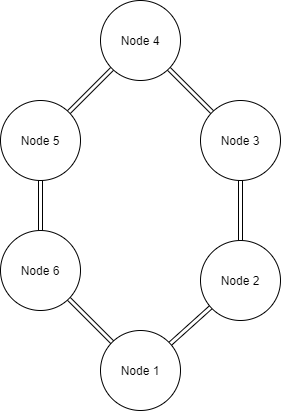
\includegraphics[width=\textwidth]{konklusjon/Mesh.png}
    \caption{Et tenkt maskenettverk for å dekke en hel vindturbin med seks noder. }
    \label{fig:maskenettverk}
  \end{minipage}
  \hfill
  \begin{minipage}[b]{0.45\textwidth}
    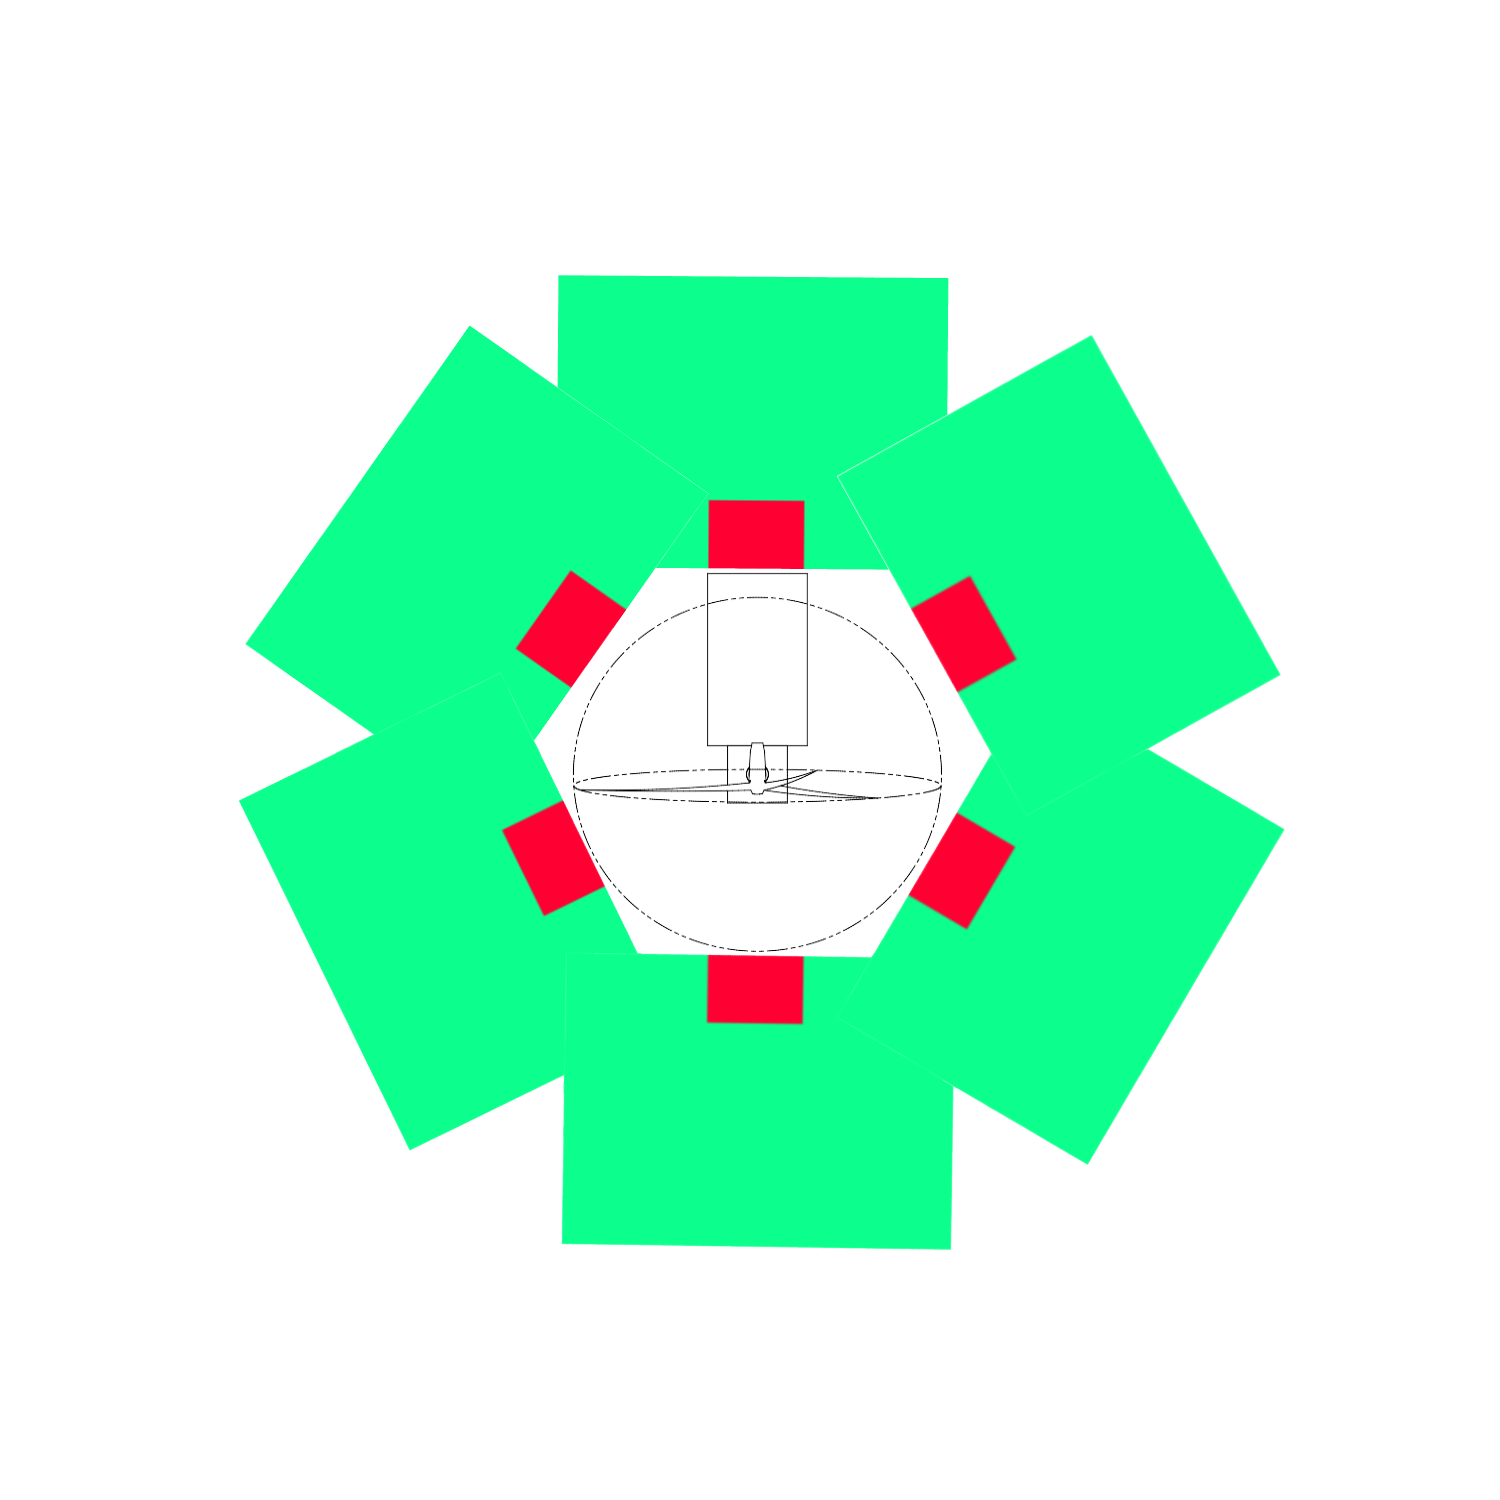
\includegraphics[width=\textwidth]{konklusjon/Nettverk.png}
    \caption{Konsept for hvordan seks kameraer kan detektere fugleaktivitet inn mot en vindturbin fra alle retninger. Det grønne området er deteksjonsområdet og rødt er boksenes plassering.}
    \label{fig:fraoven}
  \end{minipage}
\end{figure}

En hovedprosesseringsenhet kan ta inn data fra alle nodene, og bruke dette for å lage et 2D-kart over flymønstre. 
Til dette må det brukes sannsynlighet for å forsøke å modellere banene til fuglene som er detektert, sånn at man klarer å tracke en fugl fra en node til en annen. 
I informasjonsinnhentingen til dette prosjektet, ble det sett eksempler på hvor kalman-filter ble tatt i bruk for et slikt formål \cite{kalman}. 
Et maskenettverk kan potensieltsett også brukes for å detektere om en fugl har kollidert med turbinene. Dersom en fugl flyr inn mot en turbinen, uten å fly ut igjen, vil det være en reell sannsynlighet for at fuglen har kollidert.

Dette kan også hjelpe i områder uten vindkraftutbygging der man skal telle fugler på et større område. 
Dette 2D-kartet over flymønstre vil for eksempel kunne brukes for å optimalisere plasseringen av vindturbinen, dersom fuglene har en tendens til å fly over spesifikke områder innenfor deteksjonsområdet.



\subsubsection{Oppgradering av IR-sensoren}\label{sec:videreutvikling:ir-sensor}
IR-kameraet som ble brukt er et kommersielt kamera designet for å være brukervennlig. 
Dette skaper en del begrensninger rundt dataen vi får ut fra kameraet. 
Spesielt har den automatiske kalibreringen, diskutert i \autoref{sec:verifikasjon:kamera:kalibrering}, skapt problemer.  
I en videreutvikling burde dermed dette kommersielle kameraet byttes ut med kun en IR-sensor. 
Dette vil gi systemet større kontroll over rådataen fra kameraet.
En IR-sensor med lengre rekkevidde og bedre oppløsning vil også gjøre det mulig å kartlegge arter og størrelser på fugler \cite{species}. 
Dette minsker behovet for et konvensjonelt kamera, som også ville vært avhengig av å ha god sikt. 
Kunnskap om art kan også i teorien kombineres med fuglens størrelse på skjermen for å slå fast avstand, gitt at fugler av den aktuelle arten har en kjent størrelse. 
Dette vil sannsynligvis være komplisert og kreve mye testing.

\subsubsection{Ordinært bilde}\label{sec:videreutvikling:kamera}
For enkelt å kunne sjekke om dataen fra fugletelleren er rimelig, kunne det vært gunstig å supplere IR-kameraet med et ordinært kamera som kun tar bilder når IR-kameraet detekterer en fugl.
Dette bilde kan så bli sendt til databasen, og gjort tilgjengelig på nettsiden.
Dette gjør det mulig for brukeren å enkelt dobbeltsjekke dataen, i tillegg til at det gjør det mulig å kartlegge art, enten automatisk ved hjelp av maskinlæring eller av et menneske. Dette vil kun fungere på dagtid og med god sikt.

\subsubsection{Uavhengighet fra infrastruktur}\label{sec:videreutvikling:strøm}
For at brukeren skal ha større frihet ved plasseringen av produktet, er det viktig at det har sin egen strømforsyner og ikke er avhengig av å kobles til strømnettet.
Dette er spesielt viktig dersom man ønsker å overvåke et sted uten foreløpig installerte vindturbiner, da dette kan være langt unna eksisterende strømnett.
I en videreutvikling av produktet, vil det dermed være lurt å se på mulighetene for å koble produktet til et batteri, eventuelt supplert fra et lite solcellepanel eller liten vindturbin. 

Det vil også være aktuelt å utforske muligheter for å ikke være avhengig av Wi-Fi for å overføre data, slik at systemet kan brukes fritt flere steder. Dette kan for eksempel erstattets ved å bruke mobilnettverk.

\subsubsection{Programvare}\label{sec:videreutvikling:programvare}


Filtreringen av bildene hadde sine begrensninger i dette prosjektet, som diskutert i \autoref{sec:verifikasjon:programvare:filtrering}. Ettersom det også hadde vært ønskelig å ta i bruk en annen IR-sensor som nevnt i \autoref{sec:videreutvikling:ir-sensor} ville filtreringsoppgaven blitt mer utfordrende og komplisert. Flere typer filter måtte blitt tatt i bruk og kombinert for å pålitelig kunne filtrere bilder i forskjellige typer værforhold. Dette vil kunne brukes sammen med værdata fra værstasjonen slik at systemet automatisk bestemmer type filter avhengig av værforholdene. 



\subsubsection{Nettside og database}

Videreutvikling av nettsiden og databasen vil kunne være å legge til flere spesialiserte grafer for forskjellige data. 
Dersom det blir behov for et maskenettverk vil det også måtte være nødvendig å legge til funksjonalitet for å kunne støtte dette. 
Det kan være et kart der du kan se de forskjellige systemene og statistikk for hver enkelt node. 

Databasen har en svakhet, den er relativt treg. Samtidig er den meget fleksibel. 
Det finnes flere løsninger som håndterer dette, men å gå over til en database som ikke er så fleksibel mot at den blir raskere er en mulighet. 


\subsection{Bruk}

Etter at systemet er satt ut på ønsket område, vil produktet automatisk registrere fugler og værdata uten ytterligere menneskelig interaksjon. 
Produktet er svært enkelt å sette opp, og krever kun tilgang til en vanlig stikkontakt og internett. 

Produktet er i utgangspunktet vedlikeholdsfritt.
Det vil allikevel kunne oppstå situasjoner der menneskelig interaksjon er nødvendig. 
Dette kan for eksempel være dersom kameralinsen blir blokkert, eller pålen systemet står på velter. 

\subsection{Konklusjon}
Systemet bruker et IR-kamera, en prosesseringsenhet og bildebehandling for å detektere, telle og spore fugler i kameraets synsfelt. 
Systemet sender antall registrerte fugler sammen med værdata fra systemets egne sensorer til en database.
En nettside henter data fra databasen, og sorterer disse etter brukerens ønske. 
Under testing oppnåde systemet en treffrate, antall fugler korrekt registrert, på $75\%$ i klart vær. 
Systemet har lavere treffrate når det er skyer.
Dette kommer i hovedsak av den automatiske kalibreringen av IR-kameraet. 
Alle delsystemene fungerer, fra overvåking av fugleaktivitet og innsamling av værdata til presentering på en nettside.


\subsection{Takk}

Takk til vår faglige veileder Bjørn B. Larsen for god veiledning.

Takk til Institutt for Elkraftteknikk ved NTNU for lån av IR-kameraet, FLIR C3. 

Takk til tålmodige foreldre og gode venner for å lese gjennom og sjekke dokumentet.

Takk til Institutt for Elektroniske Systemer for lån av en Raspberry Pi 3B til testing. 

Takk til Torjus Bakkene ved Ascend NTNU for teknisk veiledning.

Takk til Omega verksted for teknisk veiledning og lokaler. 